\documentclass[a4paper]{exam}

\usepackage{hyperref}
\usepackage[capitalise,nameinlink]{cleveref}
\usepackage{caption}
\usepackage{graphbox}
\usepackage{multirow}
\usepackage{pythonhighlight}
\usepackage{ragged2e}
\usepackage{subcaption}
\usepackage{tabularx}
\usepackage{titling}
\usepackage{xcolor}
\usepackage{float}
\graphicspath{{Images}}

\printanswers

\title{Weekly Challenge 13: Second Shortest Path\\CS 412 Algorithms: Design and Analysis}
\author{q1-team-2}  % <==== replace with your team name for grading
\date{Habib University | Spring 2023}

\runningheader{CS 412: Algorithms}{WC13: Second Shortest Path}{\theauthor}
\runningheadrule
\runningfootrule
\runningfooter{}{Page \thepage\ of \numpages}{}

\qformat{{\large\bf \thequestion. \thequestiontitle}\hfill}
\boxedpoints

\begin{document}
\maketitle

\begin{questions}

	\titledquestion{Courier Company}

	\begin{figure*}[!h]
		\centering
		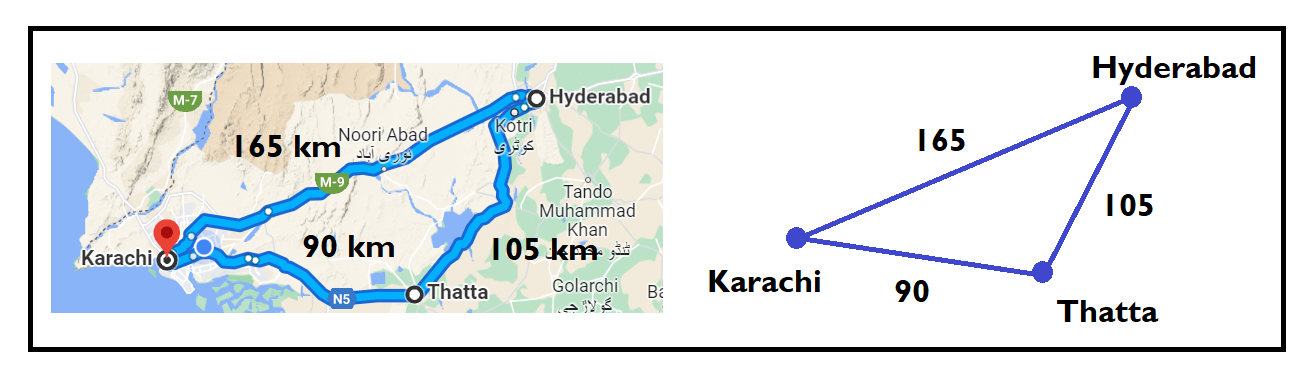
\includegraphics[width=.95\textwidth]{karachi-hyderabad-thatta.png}

		\caption{Distance Graph between 3 cities. Distances are approximate [Google Earth].}
		\label{fig:notation}
	\end{figure*}

	You are the operations manager of a courier services company. Its a festive season and there's a huge demand for delivering gifts all across Pakistan from your main operations hub located in Karachi. Your objective is to send your fleet of trucks loaded with gifts to all branch warehouses for the gifts to be delivered to local residents. There are dedicated truck routes for courier services all across the country such that branch `A' and `B' are connected if there's a direct courier route between 'A' and 'B' or there is a branch 'C' such that 'A' is connected to 'C' and 'C' is connected to 'B'.

	Your fleet of trucks has to start from the main operations hub located in Karachi and visit all branch warehouses using the minimum total distance. Note that the trucks may take varying directions.  However, you soon realize that courier trucks of other companies are also taking the same routes leading to huge traffic jams and delays in delivering gifts. Therefore, in order to save some time, you plan to choose the path that is just one step higher than the minimum distance (the 2nd minimum path) that covers all branches which may save some time.

	The objective of this problem is to compute a path that spans all branches having the overall (total) $2^{nd}$ minimum distance (in terms of the edge weights as distance), given the inputs as adjacency matrices. Note that at present, your trucks do not have to return to the main operations hub.

	\paragraph{Example} For the graph shown above, the second shortest path that visits all branches between the 3 cities has cost 255 (Karachi-Hyderabad: 165) and (Karachi-Thatta: 90). Note that the cost of the shortest path \cite{clrs} is 195, which is $not$ the required answer.

	\paragraph{Inputs and Output}
	\begin{itemize}
		\item The first line in the input file is the number of test cases.
		\item The next line is an integer $N$ ($3 \leq N \leq 100$) representing the number of branch warehouses for that case.
		\item This is followed by $N$ lines each containing $N$ integers.
		\item An integer in the $i^{th}$ line and $j^{th}$ place represents the distance [1, 1000] between branch $i$ and branch $j$.
		\item Any value greater than 1000 implies the absence of a direct link between the two branches.
		\item The output corresponding to each case is an integer which states the second minimum distance.
	\end{itemize}
	\paragraph{Task}
	You have to implement the function \texttt{second\_shortest()} in the accompanying file second\_shortest\_path.py which takes as an argument an adjacency matrix and returns the second shortest distance.
	\paragraph{Grading}
	Your submission will be automatically graded by running the pytest file which will be provided later.

	\begin{table}[]
		\centering
		\begin{tabular}{|l|l|}
			\hline
			Sample Input                  & Sample Output \\ \hline
			\texttt{2}                    &               \\ \hline
			\texttt{3}                    &               \\
			\texttt{0  990 692}           & 1169          \\
			\texttt{990  0 179}           &               \\
			\texttt{692  179 0}           &               \\
			\texttt{6}                    &               \\ \hline
			\texttt{0 13 9999 9999 39 27} & 65            \\
			\texttt{13 0 7 9999 9999 28}  &               \\
			\texttt{9999 7 0 7 9999 2}    &               \\
			\texttt{9999 9999 7 0 36 14}  &               \\
			\texttt{39 9999 9999 36 0 34} &               \\
			\texttt{27 28 2 14 34 0}      &               \\ \hline
		\end{tabular}
	\end{table}

	\begin{thebibliography}{9}
		\bibitem{clrs}
		Thomas H. Cormen, Charles E. Leiserson, Ronald L. Rivest, and Clifford Stein. 2022. \textit{Introduction to Algorithms}, Eighth Edition (8th. ed.). The MIT Press.
	\end{thebibliography}


\end{questions}

\end{document}
